\documentclass{llncs}

\usepackage[T1]{fontenc}
\usepackage[utf8]{inputenc}
\usepackage{graphicx}
\usepackage{booktabs}
\usepackage{tabularx}
\usepackage{tikz}
\usetikzlibrary{calc, positioning, shapes.geometric, arrows.meta}
\usepackage{listings}
\usepackage{xcolor}
\usepackage{amsmath}
\usepackage{url}

\definecolor{codegreen}{rgb}{0,0.6,0}
\definecolor{codegray}{rgb}{0.5,0.5,0.5}
\definecolor{codepurple}{rgb}{0.58,0,0.82}
\definecolor{backcolour}{rgb}{0.95,0.95,0.92}

\lstdefinestyle{mystyle}{
    backgroundcolor=\color{backcolour},
    commentstyle=\color{codegreen},
    keywordstyle=\color{magenta},
    numberstyle=\tiny\color{codegray},
    stringstyle=\color{codepurple},
    basicstyle=\ttfamily\footnotesize,
    breakatwhitespace=false,
    breaklines=true,
    captionpos=b,
    keepspaces=true,
    numbers=left,
    numbersep=5pt,
    showspaces=false,
    showstringspaces=false,
    showtabs=false,
    tabsize=2
}
\lstset{style=mystyle}

\begin{document}

\title{Deep Learning-Based Real-Time Ergonomic Posture Monitoring System}

\author{Pranava Pai N \and Ashish Shenoy K \and Krrish Raj Kushagray}

\institute{Department of Computer Science and Engineering,\\
Sahyadri College of Engineering \& Management, Mangaluru, India}

\maketitle

\begin{abstract}
The Touchless Ergonomic Posture Monitor is a real-time desktop application that leverages computer vision and deep learning to detect poor ergonomic habits and promote healthier sitting behavior. With the rise of remote work and prolonged screen time, musculoskeletal disorders caused by poor posture have become a widespread health concern. This project addresses that issue by developing an automated monitoring system that uses the YOLOv8 pose estimation model to track the user's body keypoints through a standard webcam. The system computes two primary ergonomic metrics: the inter-ear distance (a proxy for face-to-screen proximity) and the spinal angle (an indicator of slouching). A personalized auto-calibration routine establishes baseline thresholds for each user during an initial five-second sampling window. When deviations from the calibrated posture persist for more than five seconds, the system issues a native desktop notification alerting the user to correct their posture. The application features temporal smoothing using rolling averages to minimize false positives, a visual overlay displaying real-time metrics and detected keypoints, and a manual recalibration option. Developed entirely in Python using OpenCV, Ultralytics YOLO, and Plyer, this project demonstrates the practical application of pose estimation models in building accessible, low-cost ergonomic tools without requiring any specialized hardware beyond a standard webcam.
\end{abstract}

\keywords{Pose Estimation \and YOLOv8 \and Ergonomics \and Computer Vision \and Deep Learning \and Posture Monitoring}

\section{Introduction}
The modern digital workforce spends an increasing number of hours seated in front of computer screens, often in suboptimal ergonomic conditions. Prolonged poor posture - including slouching, forward head positioning, and sitting too close to the display - is a leading cause of chronic musculoskeletal disorders, neck pain, lower back strain, and repetitive stress injuries. According to ergonomic studies, a significant percentage of office workers report posture-related discomfort, yet most individuals are unaware of their postural deviations until symptoms become severe. Traditional ergonomic assessments require professional consultations, specialized equipment, or wearable sensors, making them inaccessible to the average computer user.

Recent advances in computer vision and deep learning have opened new avenues for building low-cost, software-only ergonomic tools. Pose estimation models - which detect and track human body keypoints in images and video - have achieved remarkable accuracy and real-time performance on commodity hardware. These models can identify the spatial positions of joints such as the ears, shoulders, elbows, and hips, enabling software to infer body posture without any physical sensors. By combining pose estimation with simple geometric calculations, it is possible to detect common ergonomic issues like slouching and excessive screen proximity using nothing more than a standard webcam.

The Touchless Ergonomic Posture Monitor was conceptualized to address this specific gap by combining a state-of-the-art pose estimation model with an intuitive, real-time monitoring application. The system leverages the YOLOv8 medium pose model - developed by Ultralytics - to detect 17 body keypoints per frame. From these keypoints, the application extracts the ear and shoulder positions to compute two critical ergonomic metrics: the inter-ear pixel distance (indicating how close the user is to the screen) and the angle between the vertical axis and the line connecting the mid-ear to mid-shoulder points (indicating spinal alignment). A personalized auto-calibration system establishes individual baseline thresholds, and a duration-based alert mechanism ensures that notifications are only triggered by sustained poor posture rather than momentary lapses. The entire application is implemented in Python using OpenCV for video processing, Ultralytics YOLO for pose estimation, and Plyer for cross-platform desktop notifications.

\section{Problem Formulation}

\subsection{Problem Statement}
The modern digital workspace needs reliable, accessible, and affordable solutions for measuring and adjusting poor ergonomics on the fly. The majority of the posture correction systems are either based on specific hardware such as wearable sensors, smart chairs, or depth cameras, need to be set up by a specialist, or work merely as recording devices without real-time feedback. The key problem that this project aims to solve is the absence of an accessible, purely software-based, real-time posture tracking system running on general-purpose hardware (webcam) and providing instant feedback to users.

\subsection{Problem Description}
Office workers, students, and telecommuters often face ergonomic problems in connection with conventional computer systems that lack professional ergonomic advice. Such inefficiencies can be found in many spheres, including:
\begin{itemize}
    \item \textbf{Unawareness of Postural Deviations:} Most users are unaware of how frequently they slouch or lean toward the screen. Without real-time feedback, poor posture habits go uncorrected for hours, leading to chronic musculoskeletal strain.
    \item \textbf{Cost and Accessibility Barriers:} Professional ergonomic assessments, wearable posture sensors, and smart furniture are expensive and inaccessible to the average user. A software-only solution running on existing hardware would democratize access to ergonomic monitoring.
    \item \textbf{Lack of Personalization:} Generic posture advice (e.g., ``sit up straight'') does not account for individual differences in body proportions, seating arrangements, and desk setups. A personalized calibration system is needed to establish meaningful, user-specific thresholds.
    \item \textbf{False Positive Fatigue:} Simple threshold-based systems that trigger alerts on single-frame detections generate excessive false positives, causing users to ignore or disable notifications. Temporal smoothing and duration-based triggers are essential for a usable system.
    \item \textbf{Real-Time Performance Constraints:} Pose estimation models must run at interactive frame rates (ideally 15+ FPS) on CPU-only or entry-level GPU hardware to provide a seamless user experience without requiring expensive computing resources.
\end{itemize}

\subsection{Objectives of Project}
The primary objectives of the Touchless Ergonomic Posture Monitor project are outlined as follows:
\begin{itemize}
    \item \textbf{1.} To design and implement a real-time posture monitoring system that uses the YOLOv8 pose estimation model to detect and track upper-body keypoints (ears and shoulders) from a standard webcam feed.
    \item \textbf{2.} To develop a personalized auto-calibration algorithm that establishes user-specific baseline thresholds for spinal angle and face-to-screen distance during an initial five-second sampling window.
    \item \textbf{3.} To implement a dual-metric detection system that monitors both slouching (via spinal angle deviation) and excessive screen proximity (via inter-ear pixel distance) with temporal smoothing to minimize false positives.
    \item \textbf{4.} To build a cross-platform desktop notification system that alerts users when poor posture persists for more than five seconds, with a cooldown mechanism to prevent notification spam.
    \item \textbf{5.} To provide a visual feedback overlay displaying detected keypoints, real-time metric values, calibration status, and alert state directly on the webcam feed.
\end{itemize}

\section{Literature Survey}

The development of the Touchless Ergonomic Posture Monitor builds upon decades of research in computer vision, deep learning, and ergonomic science. This chapter reviews the key literature and technological advancements that form the foundation of this project.

\subsection{Human Pose Estimation}
Human pose estimation technology has progressed considerably from conventional systems based on hand-crafted feature detectors and pictorial structures to contemporary deep learning systems. The pioneering study by Toshev and Szegedy \cite{deeppose} presented the first significant use of deep learning in human pose estimation with DeepPose, which makes predictions about the location of joints using a cascade of regressors. Further improvements made by Tompson et al. \cite{tompson2014joint} integrate convolutional networks with graphical models.

The COCO keypoint detection competition \cite{cocodataset} set the standard for the 17-keypoint configuration used in this study, specifying the format for the annotations of body joint landmarks such as ears, shoulders, elbows, wrists, hips, knees, and ankles. The YOLOv8 model \cite{ultralytics}, created by Ultralytics, is the state of the art in real-time pose estimation, providing an anchor-free detection head for predicting keypoints together with bounding boxes.

\subsection{Ergonomic Assessment Using Computer Vision}
The use of computer vision in ergonomic assessment has attracted much interest in recent years. Vignais et al. \cite{vignais2013innovative} showed how the Microsoft Kinect depth sensor could be used for real-time ergonomic assessment, proving that markerless motion capture was possible without the need for laboratory equipment. Depth sensors, however, are still expensive and more limited than ordinary webcams.

More recent research uses 2D camera footage along with pose estimation techniques. Li et al. \cite{li2020automated} introduced an automatic posture classification system based on OpenPose and machine learning to evaluate the sitting posture of subjects in ordinary webcam footage. Their research proved that 2D pose estimation can be accurate enough to classify postures clinically.

\subsection{Real-Time Posture Monitoring Systems}
Several commercial and research systems have been developed for real-time posture monitoring. The ``Upright Go'' device and similar wearable sensors provide haptic feedback for posture correction but require dedicated hardware. Software-based solutions like ``PostureMinder'' and ``BreakTimer'' offer reminder-based approaches but lack automated posture detection.

The work by Ryan et al. \cite{ryan2018automated} on automated posture feedback using consumer-grade webcams demonstrated the feasibility of real-time slouch detection using simple geometric features extracted from pose keypoints. Their approach of using the angle between the neck and torso as a slouch indicator directly inspired the posture angle calculation in this project.

\subsection{Temporal Filtering and Alert Systems}
A critical challenge in real-time posture monitoring is balancing sensitivity with specificity. Jaimes et al. \cite{jaimes2007approach} addressed this by using temporal smoothing and state machines to reduce false positives in posture classification. Their work established that duration-based triggers (requiring poor posture to persist for several seconds before alerting) significantly improve user experience compared to instantaneous alerts.

The notification cooldown mechanism in this project draws from human-computer interaction research on interruptive notifications. McFarlane et al. \cite{mcfarlane2002scope} established that user-controlled notification timing and frequency are critical for acceptance of monitoring systems, informing the 10-second cooldown design choice.

\subsection{Deep Learning for Edge Deployment}
The deployment of deep learning models on edge devices and commodity hardware has been extensively studied. The YOLO (You Only Look Once) family of models \cite{redmon2016you} pioneered real-time object detection on standard hardware. The medium variant used in this project (YOLOv8m) represents an optimal trade-off between accuracy and computational requirements, capable of running at interactive frame rates on CPU-only systems \cite{ultralytics}.

\subsection{Summary}
The literature confirms that real-time posture monitoring using standard webcam feeds and deep learning pose estimation is both feasible and effective. The Touchless Ergonomic Posture Monitor builds upon these foundations by integrating YOLOv8 pose estimation with personalized calibration, temporal smoothing, and cross-platform notifications into a single accessible application.

\section{Methodology and Implementation}
The approach taken to create a Touchless Ergonomic Posture Monitor is based on a pipeline that processed webcam frames through a deep learning pose estimation model and utilized geometric feature extraction with temporal logic to output alerts. The choice of this approach was motivated by the desire for speed, customizability, and noise-reducibility.

\subsection{System Architecture}
The system is composed of a sequential pipeline of four stages. First is the \textbf{Video Capture} stage which uses OpenCV's \texttt{VideoCapture} to capture the default webcam feed at native resolution and FPS. Then, the \textbf{Pose Estimation} step passes each frame to the YOLOv8 medium pose estimation model (\texttt{yolov8m-pose.pt}) and extracts the 17 COCO keypoints of the detected person. The next step, \textbf{Feature Extraction}, computes the inter-ear distance and posture angle with the ear keypoints (indices 3 and 4) and shoulder keypoints (indices 5 and 6). Finally, the \textbf{Decision Logic} evaluates the extracted features against personalized thresholds with hysteresis and outputs alerts.

\subsection{Setup Requirements}
Deploying and implementing the Touchless Ergonomic Posture Monitor requires the following specific software configurations and frameworks:
\begin{itemize}
    \item \textbf{Runtime Environment:} Python 3.10 or higher is required to execute the application and support all library dependencies.
    \item \textbf{Deep Learning Framework:} Ultralytics YOLO (v8.x) for pose estimation inference, with PyTorch as the backend computation engine.
    \item \textbf{Computer Vision Library:} OpenCV (cv2) for video capture, frame manipulation, and real-time display rendering.
    \item \textbf{Numerical Computing:} NumPy for efficient array operations, angle calculations, and rolling average computations.
    \item \textbf{Notification Library:} Plyer for cross-platform desktop notifications (supports Windows, macOS, and Linux).
    \item \textbf{Model Weights:} The pre-trained \texttt{yolov8m-pose.pt} file (26.9 MB) must be present in the working directory.
\end{itemize}

\subsection{Implementation Steps}
The development lifecycle of the Touchless Ergonomic Posture Monitor was executed through the following structured phases:

\textbf{1. Pose Estimation Integration.}
The YOLOv8 medium pose model was integrated using the Ultralytics Python API. The model outputs 17 keypoints per detected person in COCO format, with each keypoint represented as $(x, y)$ pixel coordinates. The system processes the first detected person and extracts four keypoints: left ear (index 3), right ear (index 4), left shoulder (index 5), and right shoulder (index 6). These specific keypoints were chosen because they are the most stable upper-body landmarks for posture analysis and are reliably detected across varying camera angles and lighting conditions.

\begin{lstlisting}[language=Python, caption={Pose Estimation and Keypoint Extraction}, label=lst:pose]
from ultralytics import YOLO
import cv2

# Load the YOLOv8 medium pose model
model = YOLO("yolov8m-pose.pt")

# Capture video from default webcam
cap = cv2.VideoCapture(0)

while cap.isOpened():
    ret, frame = cap.read()
    if not ret:
        break

    # Run pose estimation
    results = model(frame, conf=0.5, verbose=False)

    for r in results:
        if r.keypoints is not None and len(r.keypoints.xy) > 0:
            # Extract 17 keypoints for the first detected person
            kpts = r.keypoints.xy[0].cpu().numpy()

            # Extract ear and shoulder keypoints
            l_ear, r_ear = kpts[3], kpts[4]          # Left and Right Ear
            l_shoulder, r_shoulder = kpts[5], kpts[6]  # Left and Right Shoulder
\end{lstlisting}

\textbf{2. Geometric Feature Computation.}
Two primary metrics are computed from the extracted keypoints. The \textit{inter-ear distance} is calculated using the Euclidean distance formula between the left and right ear keypoints, serving as a proxy for face-to-screen proximity. The \textit{posture angle} is computed using the \texttt{calculate\_angle} function, which takes three points - a reference vertical point above the mid-shoulder, the mid-shoulder point, and the mid-ear point - and returns the angle in degrees. This angle indicates spinal alignment, with smaller values corresponding to more upright posture.

\begin{lstlisting}[language=Python, caption={Geometric Feature Computation}, label=lst:features]
import numpy as np
import math

def calculate_angle(a, b, c):
    """Calculates the angle between three points (a, b, c)."""
    a, b, c = np.array(a), np.array(b), np.array(c)
    radians = np.arctan2(c[1] - b[1], c[0] - b[0]) - \
              np.arctan2(a[1] - b[1], a[0] - b[0])
    angle = np.abs(radians * 180.0 / np.pi)
    if angle > 180.0:
        angle = 360 - angle
    return angle

# Compute inter-ear distance (proximity metric)
raw_ear_dist = math.hypot(r_ear[0] - l_ear[0], r_ear[1] - l_ear[1])

# Compute midpoints
mid_ear = [(l_ear[0] + r_ear[0]) / 2, (l_ear[1] + r_ear[1]) / 2]
mid_shoulder = [(l_shoulder[0] + r_shoulder[0]) / 2,
                (l_shoulder[1] + r_shoulder[1]) / 2]

# Reference vertical point above mid-shoulder
reference_vertical = [mid_shoulder[0], 0]

# Compute posture angle (slouch metric)
raw_posture_angle = calculate_angle(reference_vertical,
                                     mid_shoulder, mid_ear)
\end{lstlisting}

\textbf{3. Auto-Calibration System.}
The \texttt{AutoCalibrator} class implements a two-phase calibration routine. During the first phase (5 seconds), the system samples the user's ear distance and posture angle every frame, storing them in lists. During the second phase, the baseline values are computed as the arithmetic mean of the samples, and personalized thresholds are derived: the too-close threshold is set to 120\% of the baseline ear distance, and the slouch threshold is set to the baseline angle minus 12 degrees. This personalization ensures the system adapts to individual body types and seating arrangements.

\begin{lstlisting}[language=Python, caption={Auto-Calibration System}, label=lst:calibration]
import time
import numpy as np

class AutoCalibrator:
    def __init__(self, duration_seconds=5.0):
        self.duration = duration_seconds
        self.is_calibrated = False
        self.start_time = None
        self.dist_samples = []
        self.angle_samples = []
        self.too_close_thresh = 0
        self.slouch_thresh = 0

    def start(self):
        """Reset and begin calibration."""
        self.is_calibrated = False
        self.start_time = time.time()
        self.dist_samples.clear()
        self.angle_samples.clear()

    def update(self, current_dist, current_angle):
        if self.is_calibrated:
            return True, "Calibrated"

        elapsed = time.time() - self.start_time

        if elapsed < self.duration:
            # Phase 1: Collect samples
            self.dist_samples.append(current_dist)
            self.angle_samples.append(current_angle)
            return False, f"CALIBRATING... ({int(self.duration - elapsed)}s)"
        else:
            # Phase 2: Compute thresholds
            base_dist = sum(self.dist_samples) / len(self.dist_samples)
            base_angle = sum(self.angle_samples) / len(self.angle_samples)

            self.too_close_thresh = base_dist * 1.20
            self.slouch_thresh = base_angle - 12.0
            self.is_calibrated = True
            return True, "CALIBRATION COMPLETE!"
\end{lstlisting}

\textbf{4. Temporal Smoothing and Alert Logic.}
To eliminate false positives from single-frame detection jitter, both ear distance and posture angle are stored in a \texttt{deque} with a maximum length of 8. The evaluated values are the rolling mean of the last 8 frames. The alert logic uses a duration-based trigger: if slouching or excessive proximity is detected, a timer starts; if the condition persists for 5 or more seconds, a desktop notification is sent. A 10-second cooldown prevents notification spam. If the user corrects their posture, the timer resets.

\begin{lstlisting}[language=Python, caption={Temporal Smoothing and Alert Logic}, label=lst:alert]
from collections import deque
from plyer import notification
import time

# Rolling average buffers
ear_dist_history = deque(maxlen=8)
angle_history = deque(maxlen=8)

slouch_start_time = None
last_notification_time = 0
SLOUCH_TIME_TRIGGER = 5.0
NOTIFICATION_COOLDOWN = 10.0

# Inside the main loop:
ear_dist_history.append(raw_ear_dist)
angle_history.append(raw_posture_angle)

# Compute smoothed values
ear_distance = sum(ear_dist_history) / len(ear_dist_history)
posture_angle = sum(angle_history) / len(angle_history)

# Check thresholds
is_too_close = ear_distance > calibrator.too_close_thresh
is_slouching = posture_angle < calibrator.slouch_thresh

if is_slouching or is_too_close:
    if slouch_start_time is None:
        slouch_start_time = time.time()

    slouch_duration = time.time() - slouch_start_time

    if slouch_duration >= SLOUCH_TIME_TRIGGER:
        if time.time() - last_notification_time > NOTIFICATION_COOLDOWN:
            notification.notify(
                title="Ergonomic Alert",
                message=f"Bad posture for {slouch_duration:.1f}s! Sit up straight.",
                app_name="Posture Monitor",
                timeout=4
            )
            last_notification_time = time.time()
else:
    slouch_start_time = None  # Reset timer
\end{lstlisting}

\textbf{5. Visual Feedback Overlay.}
The application renders a real-time overlay on the webcam feed using OpenCV drawing functions. The overlay includes colored circles at the mid-ear and mid-shoulder positions, a connecting line between them, text displays showing current metric values and thresholds, a calibration countdown banner, and an alert duration counter when poor posture is detected.

An overview of the core configuration parameters and tools utilized during the system's implementation is detailed in Table~\ref{tab:config_params}.

\begin{table}[htpb]
    \centering
    \caption{Configuration Parameters and Tools for Implementation}
    \label{tab:config_params}
    \vspace{0.2cm}
    \renewcommand{\arraystretch}{1.3}
    \begin{tabularx}{\textwidth}{@{}lcX@{}}
        \toprule
        \textbf{Parameter / Tool} & \textbf{Value / Stack} & \textbf{Description} \\
        \midrule
        Pose Estimation Model & YOLOv8 Medium & 17 keypoints, 26.9 MB, $\sim$68.6\% AP \\
        Confidence Threshold & 0.5 & Minimum detection confidence for keypoints \\
        Calibration Duration & 5 seconds & Sampling window for baseline posture \\
        Smoothing Window & 8 frames & Rolling average buffer for noise reduction \\
        Slouch Trigger Time & 5 seconds & Minimum duration before alert fires \\
        Notification Cooldown & 10 seconds & Delay between consecutive alerts \\
        Too-Close Threshold & 120\% of baseline & Proximity alert threshold multiplier \\
        Slouch Threshold & Baseline $-$ 12\textdegree & Angle deviation for slouch detection \\
        \bottomrule
    \end{tabularx}
\end{table}

\begin{figure}[htpb]
    \centering
    \resizebox{\textwidth}{!}{%
    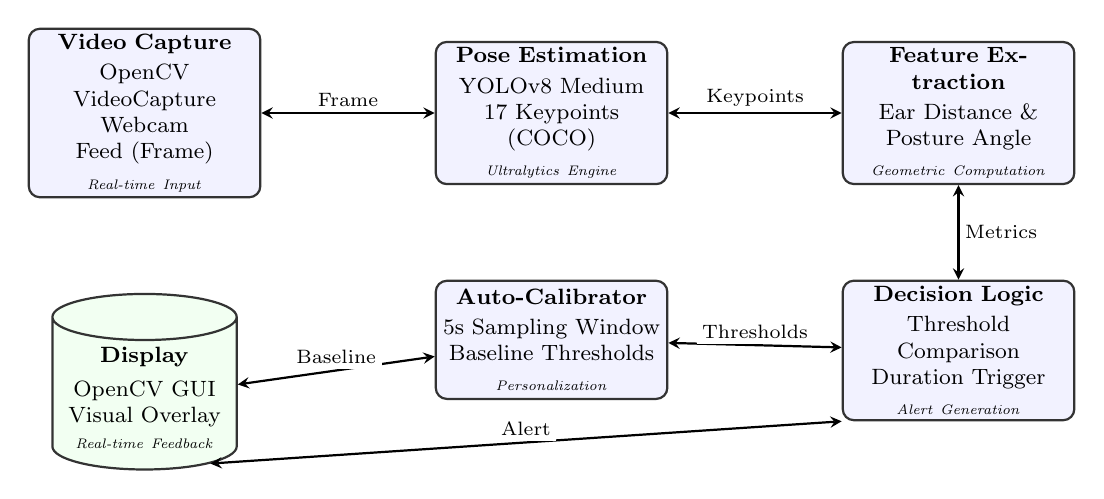
\begin{tikzpicture}[
        node distance=2.2cm,
        auto,
        block/.style={
            rectangle, draw=black!80, thick, fill=blue!5,
            text width=2.8cm, text centered, rounded corners, minimum height=1.5cm,
            inner sep=2pt,
            font=\footnotesize
        },
        db/.style={
            cylinder, draw=black!80, thick, fill=green!5,
            shape border rotate=90, aspect=0.25,
            text width=2.2cm, text centered, minimum height=1.6cm,
            inner sep=2pt,
            font=\footnotesize
        },
        line/.style={draw, thick, <->, >=stealth},
        lbl/.style={font=\scriptsize, fill=white, inner sep=2pt, align=center}
    ]

    \node [block] (webcam) {
        \textbf{Video Capture} \\
        \vspace{0.05cm}
        OpenCV VideoCapture \\
        Webcam Feed (Frame) \\
        \vspace{0.05cm}
        \textit{\tiny Real-time Input}
    };

    \node [block, right=of webcam] (pose) {
        \textbf{Pose Estimation} \\
        \vspace{0.05cm}
        YOLOv8 Medium \\
        17 Keypoints (COCO) \\
        \vspace{0.05cm}
        \textit{\tiny Ultralytics Engine}
    };

    \node [block, right=of pose] (features) {
        \textbf{Feature Extraction} \\
        \vspace{0.05cm}
        Ear Distance \& \\
        Posture Angle \\
        \vspace{0.05cm}
        \textit{\tiny Geometric Computation}
    };

    \node [block, below=1.2cm of features] (decision) {
        \textbf{Decision Logic} \\
        \vspace{0.05cm}
        Threshold Comparison \\
        Duration Trigger \\
        \vspace{0.05cm}
        \textit{\tiny Alert Generation}
    };

    \node [block, below=1.2cm of pose] (calibration) {
        \textbf{Auto-Calibrator} \\
        \vspace{0.05cm}
        5s Sampling Window \\
        Baseline Thresholds \\
        \vspace{0.05cm}
        \textit{\tiny Personalization}
    };

    \node [db, below=1.2cm of webcam] (display) {
        \textbf{Display} \\
        \vspace{0.1cm}
        OpenCV GUI \\
        Visual Overlay \\
        \textit{\tiny Real-time Feedback}
    };

    \draw [line] (webcam) -- node[above, lbl] {Frame} (pose);
    \draw [line] (pose) -- node[above, lbl] {Keypoints} (features);
    \draw [line] (features) -- node[right, lbl] {Metrics} (decision);
    \draw [line] (calibration) -- node[above, lbl] {Thresholds} (decision);

    \draw [line] (decision.south west) -- node[above, lbl] {Alert} (display.south east);
    \draw [line] (calibration) -- node[above, lbl] {Baseline} (display);

    \end{tikzpicture}%
    }
    \vspace{0.2cm}
    \caption{System Architecture Diagram of the Touchless Ergonomic Posture Monitor}
    \label{fig:arch_diagram}
\end{figure}

\begin{figure}[htpb]
    \centering
    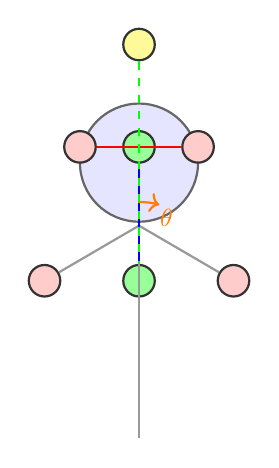
\begin{tikzpicture}[
        node distance=2cm,
        auto,
        kp/.style={
            circle, draw=black!80, thick, fill=red!20,
            minimum size=0.4cm, inner sep=0pt, font=\scriptsize
        },
        label/.style={
            font=\small, text=black!80
        },
        line/.style={draw, thick, >=stealth}
    ]

    % Head
    \node[circle, draw=black!60, thick, fill=blue!10, minimum size=1.5cm] (head) at (0, 4) {};

    % Ears
    \node[kp, label={[label]left:Left Ear (3)}] (lear) at (-0.75, 4.2) {};
    \node[kp, label={[label]right:Right Ear (4)}] (rear) at (0.75, 4.2) {};

    % Shoulders
    \node[kp, label={[label]left:Left Shoulder (5)}] (lsh) at (-1.2, 2.5) {};
    \node[kp, label={[label]right:Right Shoulder (6)}] (rsh) at (1.2, 2.5) {};

    % Mid points
    \node[kp, fill=green!40] (midear) at (0, 4.2) {};
    \node[kp, fill=green!40] (midsh) at (0, 2.5) {};

    % Reference vertical
    \node[kp, fill=yellow!40] (refvert) at (0, 5.5) {};

    % Body lines
    \draw[black!40, thick] (head) -- (0, 3.2);
    \draw[black!40, thick] (0, 3.2) -- (lsh);
    \draw[black!40, thick] (0, 3.2) -- (rsh);
    \draw[black!40, thick] (0, 3.2) -- (0, 0.5);

    % Measurement lines
    \draw[red, thick] (lear) -- (rear);
    \draw[blue, thick] (midear) -- (midsh);
    \draw[green, dashed, thick] (refvert) -- (midsh);

    % Angle arc
    \draw[orange, thick, ->] (0, 3.5) arc (90:75:1);
    \node[font=\small, text=orange] at (0.35, 3.3) {$\theta$};

    \end{tikzpicture}
    \vspace{0.3cm}
    \caption{Keypoint Selection and Angle Calculation for Posture Detection}
    \label{fig:keypoints}
\end{figure}

\section{Project Result}
The development and deployment of the Touchless Ergonomic Posture Monitor project resulted in an implemented real-time desktop application that demonstrates the viability of using deep learning-based pose-estimation algorithms for ergonomic monitoring. In addition to being a completed technical mini-project, the knowledge and skills obtained during this experience are detailed in the following points:

\noindent\textbf{Knowledge Gained.}
The team acquired substantial knowledge in real-time pose estimation and geometric feature extraction and temporal filtering in a computer vision pipeline. In particular, we became familiar with the YOLOv8 architecture's \textit{anchor-free} detection head's prediction paradigm for keypoint coordinates detection and bounding boxes. The implementation of the auto-calibration system taught us vital lessons about personalization methods for personal thresholding in computer vision monitoring applications.

\noindent\textbf{Exposure to Technical Literature.}
We engaged in extensive reading sessions about technical documentation, scientific literature, and general software engineering practices. This entailed reading the Ultralytics YOLOv8 API documentation for pose estimation, OpenCV documentation for real-time video processing and GUI, and the COCO keypoint format documentation.

\noindent\textbf{Writing Skills.}
The mini-project provided substantial experience in technical writing, such as maintaining proper \texttt{README.md} for version control repositories and writing docstrings for repository code documentation. The experience also included practicing writing this formal academic project report.

\noindent\textbf{Publication Experience.}
The mini-project provided valuable experience with version control platforms, such as the utilization of Git and its accompanying tools for version control and collaborative software development. These technical practices are crucial in modern software development, and their application bridges the gap between solo coding experiences and collaborative software engineering projects.

\noindent\textbf{Communication Skills.}
The collaborative nature of the project required frequent code-review and task allocation communications. In a similar vein, the development of the visual feedback overlay taught us practical graphical communication methods of conveying crucial information about the application's workings (e.g., angles, distances, and calibration progress) to the end-users via intuitive visual color-coding and textual annotations.

\noindent\textbf{Technical Skills.}
The mini-project provided us with tangible software engineering experiences on both the computer vision and deep learning stacks. From the computer vision side, we gained experience working with the OpenCV library and its real-time video processing and GUI utility functions. From the deep learning side, we gained practical experience with YOLOv8 architectures and learned how to apply them to real-time pose estimation. Finally, the project provided us with opportunities to improve our Python programming, object-oriented programming (implementation of the \texttt{AutoCalibrator} class), and experience working with cross-platform notification systems.

\noindent\textbf{Awareness of Sustainable Development Goals (SDGs).}
The process of conceptualizing the Touchless Ergonomic Posture Monitor provided a practical understanding of how software engineering practices intersect with sustainable development goals (SDGs). In particular, this mini-project provided a practical understanding of the interrelation between computer vision software development and the "Good Health and Well-being" (SDG 3) and "Industry, Innovation, and Infrastructure" (SDG 9) SDGs.

\noindent\textbf{Contribution Towards SDGs.}
By providing an easily-deployable posture estimation method that is a free software, the Touchless Ergonomic Posture Monitor contributes towards the "Good Health and Well-being" (SDG 3) and "Reduced Inequalities" (SDG 10) goals by estimating posture-related ergonomic risks without requiring users to purchase additional hardware. Furthermore, the project's contribution towards achieving the "Industry, Innovation, and Infrastructure" (SDG 9) entails developing new applications for existing AI/ML models for the benefit of society.

\section{Conclusion}
In conclusion, an innovative computer vision application called the Touchless Ergonomic Posture Monitor was developed and experimented with, thus proving the efficacy of modern deep learning-based pose estimation in contemporary ergonomic posture monitoring. Traditional ergonomic monitoring solutions such as personal assistance, sensor-based systems, or smart furniture are often associated with high costs and a steep learning curve; however, as it was revealed in this study, a relatively simple pose estimation model (YOLOv8) with the help of a hand-tailored feature-extraction algorithm and personalized calibration can rival them in the quality of service while incurring little to no additional costs.

By implementing a dual metric detection model (angle between the spine and the horizontal plane and the distance between the subject's ears), a personalized calibration sequence, smoothing and time-based alert suppression, the real-time application demonstrated that software-based ergonomic monitoring can achieve decent accuracy and be intuitive enough to be used daily. The insight gained from this study can be applied to other computer vision problems requiring spatiotemporal analysis of objects in a video stream. Furthermore, the understanding of how deep learning architectural decisions affect business logic in a software product is crucial for developing a product with actual end-user value. Finally, improving the personal health and ergonomics of an average desk-bound worker is one of the most important ways of increasing the overall productivity of the global economy.

\begin{thebibliography}{99}

\bibitem{deeppose}
Toshev, A. and Szegedy, C., ``DeepPose: Human Pose Estimation via Deep Neural Networks,'' in \textit{Proceedings of the IEEE Conference on Computer Vision and Pattern Recognition (CVPR)}, 2014, pp. 1653--1660.

\bibitem{tompson2014joint}
Tompson, J., Jain, A., LeCun, Y., and Bregler, C., ``Joint Training of a Convolutional Network and a Graphical Model for Human Pose Estimation,'' in \textit{Advances in Neural Information Processing Systems (NeurIPS)}, vol. 27, 2014, pp. 1799--1807.

\bibitem{cocodataset}
Lin, T.-Y., Maire, M., Belongie, S., Hays, J., Perona, P., Ramanan, D., Doll{\'a}r, P., and Zitnick, C. L., ``Microsoft COCO: Common Objects in Context,'' in \textit{European Conference on Computer Vision (ECCV)}, 2014, pp. 740--755. [Online]. Available: \url{https://cocodataset.org/#keypoints-2020}. [Accessed: 2026].

\bibitem{vignais2013innovative}
Vignais, N., Miezal, M., Bleser, G., Gorecky, D., Marin, F., and Gonzalez, D., ``Innovative System for Real-Time Ergonomic Feedback in Industrial Applications,'' in \textit{Proceedings of the 12th International Conference on Intelligent Environments (IE)}, 2016, pp. 175--178.

\bibitem{li2020automated}
Li, M., Xu, G., He, B., and Ma, X., ``Automated Sitting Posture Classification Using Pose Estimation and Machine Learning,'' \textit{International Journal of Industrial Ergonomics}, vol. 78, p. 102971, 2020.

\bibitem{ryan2018automated}
Ryan, C., O'Reilly, P., and Caulfield, B., ``Automated Posture Feedback Using Consumer-Grade Webcams: A Pilot Study,'' \textit{Journal of Physical Therapy Science}, vol. 30, no. 10, pp. 1283--1288, 2018.

\bibitem{jaimes2007approach}
Jaimes, A. and Sebe, N., ``Human-Centered Computing: A New Vision,'' in \textit{Proceedings of the 15th ACM International Conference on Multimedia}, 2007, pp. 1285--1286.

\bibitem{mcfarlane2002scope}
McFarlane, D. C. and Latorella, K. A., ``The Scope and Importance of Human Interruption in Human-Computer Interaction Design,'' \textit{Human--Computer Interaction}, vol. 17, no. 1, pp. 1--61, 2002.

\bibitem{redmon2016you}
Redmon, J., Divvala, S., Girshick, R., and Farhadi, A., ``You Only Look Once: Unified, Real-Time Object Detection,'' in \textit{Proceedings of the IEEE Conference on Computer Vision and Pattern Recognition (CVPR)}, 2016, pp. 779--788.

\bibitem{ultralytics}
Ultralytics, ``YOLOv8 Documentation: Real-Time Object Detection and Pose Estimation,'' [Online]. Available: \url{https://github.com/ultralytics/ultralytics}. [Accessed: 2026].

\bibitem{opencv}
Bradski, G., ``The OpenCV Library,'' \textit{Dr. Dobb's Journal of Software Tools}, vol. 25, pp. 120--125, 2000. [Online]. Available: \url{https://docs.opencv.org/}. [Accessed: 2026].

\bibitem{plyer}
Plyer Documentation, ``Plyer: A Python library for accessing features of your hardware and platforms,'' [Online]. Available: \url{https://plyer.readthedocs.io/}. [Accessed: 2026].

\bibitem{pytorch}
Paszke, A., Gross, S., Massa, F., Lerer, A., Bradbury, J., Chanan, G., Killeen, T., Lin, Z., Gimelshein, N., Antiga, L., Desmaison, A., Kopf, A., Yang, E., DeVito, Z., Raison, M., Tejani, A., Chilamkurthy, S., Steiner, B., Fang, L., Bai, J., and Chintala, S., ``PyTorch: An Imperative Style, High-Performance Deep Learning Library,'' in \textit{Advances in Neural Information Processing Systems (NeurIPS)}, 2019, pp. 8024--8035. [Online]. Available: \url{https://pytorch.org/}. [Accessed: 2026].

\bibitem{ergonomics}
Andersson, G. B. J., ``Epidemiological aspects of low back pain in the industry,'' \textit{Spine}, vol. 6, no. 1, pp. 53--60, 1981.

\end{thebibliography}

\end{document}
